\documentclass[tikz,border=8pt]{standalone}
% Shared look for every TikZ diagram. Load with % Shared look for every TikZ diagram. Load with % Shared look for every TikZ diagram. Load with \input{../../tools/tikz-style.tex}
\usepackage[T1]{fontenc}
\usepackage{lmodern}
\renewcommand{\sfdefault}{lmr}  % diagrams use the same serif as the text
\usetikzlibrary{arrows.meta, positioning, shapes.geometric, calc, fit, backgrounds}
\definecolor{cblue}{HTML}{4C78A8}
\definecolor{corange}{HTML}{F58518}
\definecolor{cgreen}{HTML}{54A24B}
\definecolor{cred}{HTML}{E45756}
\definecolor{cpurple}{HTML}{B279A2}
\definecolor{cgrey}{HTML}{6B6B6B}
\tikzset{
  every picture/.style={font=\sffamily, line width=1.2pt},
  box/.style={draw=#1, fill=#1!12, rounded corners=4pt, align=center, inner sep=7pt, minimum height=1.1cm},
  box/.default=cgrey,
  arrow/.style={-{Stealth[length=3mm]}, draw=cgrey, line width=1.4pt},
  title/.style={font=\sffamily\bfseries\Large},
  note/.style={font=\sffamily\small, text=cgrey, align=center},
}
\AtBeginDocument{\hyphenpenalty=10000 \exhyphenpenalty=10000}

\usepackage[T1]{fontenc}
\usepackage{lmodern}
\renewcommand{\sfdefault}{lmr}  % diagrams use the same serif as the text
\usetikzlibrary{arrows.meta, positioning, shapes.geometric, calc, fit, backgrounds}
\definecolor{cblue}{HTML}{4C78A8}
\definecolor{corange}{HTML}{F58518}
\definecolor{cgreen}{HTML}{54A24B}
\definecolor{cred}{HTML}{E45756}
\definecolor{cpurple}{HTML}{B279A2}
\definecolor{cgrey}{HTML}{6B6B6B}
\tikzset{
  every picture/.style={font=\sffamily, line width=1.2pt},
  box/.style={draw=#1, fill=#1!12, rounded corners=4pt, align=center, inner sep=7pt, minimum height=1.1cm},
  box/.default=cgrey,
  arrow/.style={-{Stealth[length=3mm]}, draw=cgrey, line width=1.4pt},
  title/.style={font=\sffamily\bfseries\Large},
  note/.style={font=\sffamily\small, text=cgrey, align=center},
}
\AtBeginDocument{\hyphenpenalty=10000 \exhyphenpenalty=10000}

\usepackage[T1]{fontenc}
\usepackage{lmodern}
\renewcommand{\sfdefault}{lmr}  % diagrams use the same serif as the text
\usetikzlibrary{arrows.meta, positioning, shapes.geometric, calc, fit, backgrounds}
\definecolor{cblue}{HTML}{4C78A8}
\definecolor{corange}{HTML}{F58518}
\definecolor{cgreen}{HTML}{54A24B}
\definecolor{cred}{HTML}{E45756}
\definecolor{cpurple}{HTML}{B279A2}
\definecolor{cgrey}{HTML}{6B6B6B}
\tikzset{
  every picture/.style={font=\sffamily, line width=1.2pt},
  box/.style={draw=#1, fill=#1!12, rounded corners=4pt, align=center, inner sep=7pt, minimum height=1.1cm},
  box/.default=cgrey,
  arrow/.style={-{Stealth[length=3mm]}, draw=cgrey, line width=1.4pt},
  title/.style={font=\sffamily\bfseries\Large},
  note/.style={font=\sffamily\small, text=cgrey, align=center},
}
\AtBeginDocument{\hyphenpenalty=10000 \exhyphenpenalty=10000}

\begin{document}
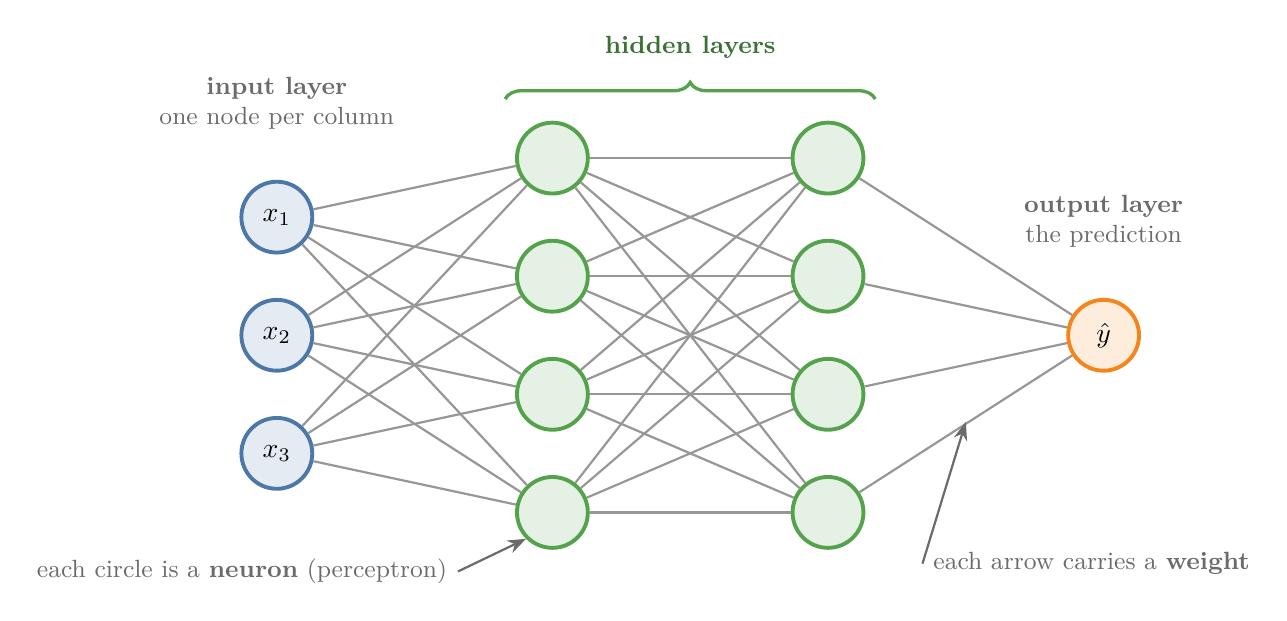
\begin{tikzpicture}[neuron/.style={circle, draw=#1, fill=#1!15, minimum size=0.9cm, line width=1.4pt}, w/.style={draw=cgrey!70, line width=0.8pt}]
  \foreach \y [count=\i] in {1.5,0,-1.5} \node[neuron=cblue] (i\i) at (0,\y) {$x_\i$};
  \foreach \y [count=\i] in {2.25,0.75,-0.75,-2.25} \node[neuron=cgreen] (a\i) at (3.5,\y) {};
  \foreach \y [count=\i] in {2.25,0.75,-0.75,-2.25} \node[neuron=cgreen] (b\i) at (7,\y) {};
  \node[neuron=corange] (o) at (10.5,0) {$\hat{y}$};
  \foreach \i in {1,2,3} \foreach \j in {1,2,3,4} \draw[w] (i\i) -- (a\j);
  \foreach \i in {1,2,3,4} \foreach \j in {1,2,3,4} \draw[w] (a\i) -- (b\j);
  \foreach \i in {1,2,3,4} \draw[w] (b\i) -- (o);
  \node[note, above=0.5cm of i1] {\textbf{input layer}\\one node per column};
  \node[note, text=cgreen!70!black] at (5.25,3.65) {\textbf{hidden layers}};
  \node[note, above=0.5cm of o] {\textbf{output layer}\\the prediction};
  \draw[cgreen, decorate, decoration={brace, amplitude=6pt}] (2.9,3.0) -- (7.6,3.0);
  % call-outs
  \node[note, anchor=west] (wn) at (8.2,-2.9) {each arrow carries a \textbf{weight}};
  \draw[-{Stealth}, cgrey, line width=0.8pt] (wn.west) -- (8.75,-1.1);
  \node[note, anchor=east] (nn) at (2.3,-3.0) {each circle is a \textbf{neuron} (perceptron)};
  \draw[-{Stealth}, cgrey, line width=0.8pt] (nn.east) -- (a4.south west);
\end{tikzpicture}
\end{document}
